\begin{frame}[noframenumbering,plain]
    \setcounter{framenumber}{1}
    \maketitle
\end{frame}

%[shrink=5]

%\begin{frame}
%\frametitle{Актуальность}
%Способы перемещения роботов в жидкости:
%\begin{itemize}
%	\item Гребные винты. Самый распространенный способ передвижения.
%	\item Изменение формы тела. 
%	\item Реакивный привод.
%	\item Действие внутренних механизмов.		
%\end{itemize}	
%
%\begin{minipage}[t]{0.47\linewidth}
%	\center{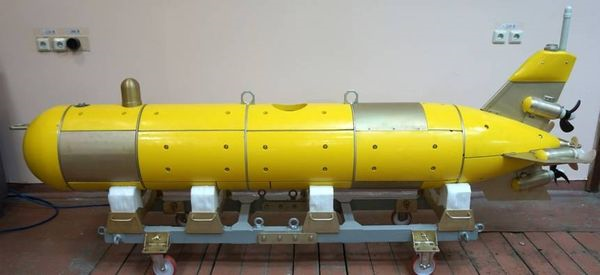
\includegraphics[height=24mm]{ScrewRobot.png}}
%\end{minipage}
%\hfill
%\begin{minipage}[t]{0.47\linewidth}
%	\center{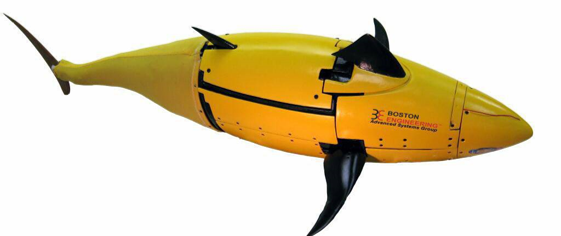
\includegraphics[height=24mm]{FishRobot.png}}
%\end{minipage}	
%\vspace{3mm}
%
%\begin{minipage}[t]{0.47\linewidth}
%	\center{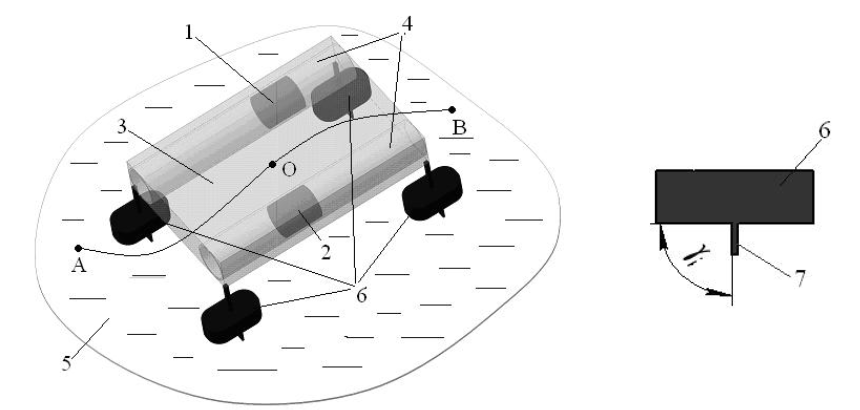
\includegraphics[height=22mm]{JatsunRobot.png}}
%\end{minipage}
%\hfill
%\begin{minipage}[t]{0.47\linewidth}
%	\center{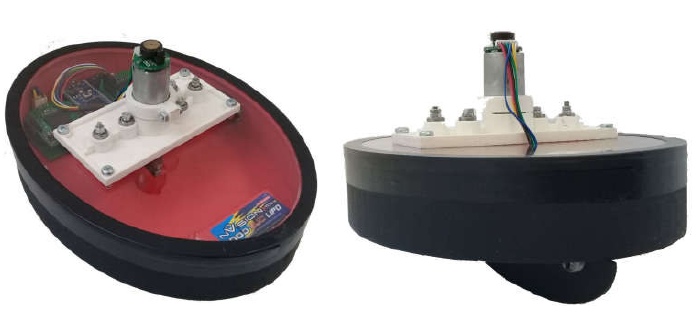
\includegraphics[height=22mm]{TolikRobot.png}}
%\end{minipage}
%
%\end{frame}	

\begin{frame}
\frametitle{Основные работы по тематике исследования}

%\begin{itemize}
\textbf{Модель в рамках идеальной жидкости.} %Показана возможность неограниченного продвижения при наличии анизотропии присоединенных масс. 

В.В. Козлов, С.М. Рамоданов, Д.А. Онищенко.
%\end{itemize}

\textbf{Заданный закон сопротивления.} 

Ф.Л. Черноусько, Н.Н. Болотник, С.Ф. Яцун.

\textbf{Совместное решения уравнений Навье-Стокса и уравнений динамики твердого тела.} 

В.А. Тененев, С.М. Рамоданов, Е.В. Ветчанин.

%\item Влияние вязкости на самопродвижение твердого тела с движущейся внутри него массой. S. Childress

\textbf{Исследование движения роботов различной формы, приводимых в движение внутренними механизмами.} 

Е.В. Ветчанин, И.С. Мамаев, А.А. Килин, А.И. Кленов, S. Childress, Ph. Tallapragada, B. Pollard.

%\item Работы Ф. Таллапрагада с соавторами -- сложная модель движения с вихреобразованием.

\vspace{3mm}

\begin{minipage}[t]{0.47\linewidth}
%	\vspace{-3mm}
	\center{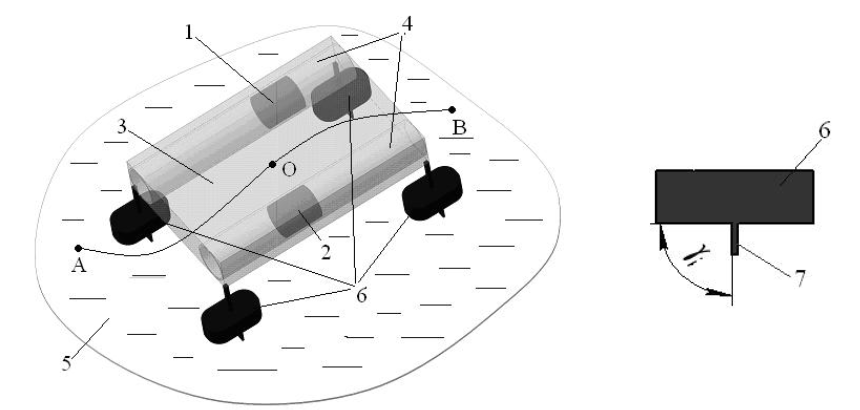
\includegraphics[width=0.9\linewidth]{JatsunRobot.png}} \\
%	\center{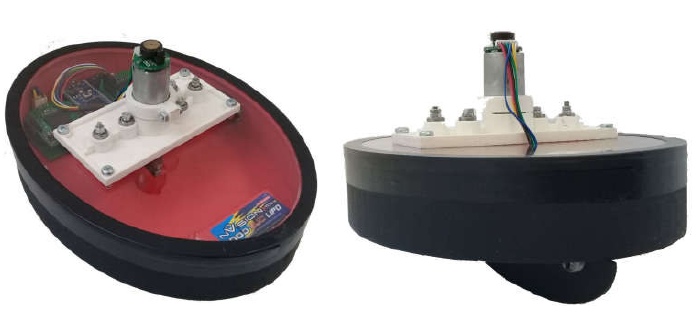
\includegraphics[height=15mm]{TolikRobot.png}}
\end{minipage}
\hfill	
\begin{minipage}[t]{0.47\linewidth}
%	\vspace{3mm}
	\center{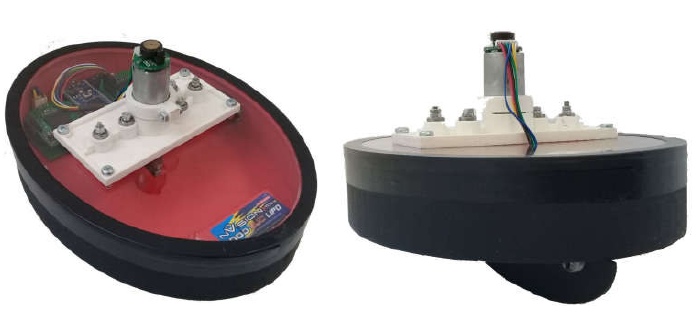
\includegraphics[width=0.9\linewidth]{TolikRobot.png}}
\end{minipage}



%\item Подробный обзор работ, посвященных движению твердого тела в жидкости, используя внутренние механизмы:

%Ветчанин Е. В., Килин А. А., Управляемое движение твердого тела с внутренними механизмами в идеальной несжимаемой жидкости, Труды Математического института имени В. А. Стеклова, 2016, т. 295, с. 321-351
%\item Экспериментальные работы: А.А. Килин, А.И. Кленов, В.А. Тененев. Управление движением тела с помощью внутренних масс в вязкой жидкости.		
%\end{itemize}

\end{frame}

\begin{frame}
\frametitle{Цель и задачи работы}
%\footnotesize

\textbf{Целью} данной работы является исследование принципов движения роботов в жидкости, управляемых внутренними механизмами и разработка алгоритмов управления их движением.


\textbf{Объекты исследования:} безвинтовой подводный робот в форме эллипсоида и безвинтовой надводный робот с острой кромкой.


\textbf{Задачи}:
\begin{itemize}
	\item Построение математической модели движения роботов в жидкости за счет изменения внутреннего гиростатического момента для каждого из объектов. %: безвинтового подводного робота в форме эллипсоида в жидкости и недеформируемого водного робота с острой кромкой.
	\item Разработка алгоритмов управления для реализации движения рассматриваемых роботов в жидкости%: безвинтового подводного робота в форме эллипсоида и недеформируемого водного робота с острой кромкой.
	\item Разработка конструкции и прототипов рассматриваемых роботов%: безвинтового подводного робота в форме эллипсоида и недеформируемого водного робота с острой кромкой; разработка систем управления.
	\item Проведение натурных экспериментов и исследования влияния режимов работы механизма на динамику рассматриваемых роботов%: безвинтового подводного робота в форме эллипсоида и недеформируемого водного робота с острой кромкой.
	\item Сравнение экспериментальных данных с результатами численного моделирования для каждого из объектов. %безвинтового подводного робота в форме эллипсоида и недеформируемого водного робота с острой кромкой.
\end{itemize}
\end{frame}

\begin{frame}
    \frametitle{Положения, выносимые на защиту}
%\small    
    \begin{itemize}
        \item Математическая модель движения в жидкости безвинтового подводного робота за счет изменения внутреннего гиростатического момента.
        \item Математическая модель движения безвинтового надводного робота, перемещающегося в жидкости за счет изменения внутреннего гиростатического момента. %с учетом вязкого трения.
        \item Алгоритм управления движением в жидкости безвинтового подводного робота за счет изменения внутреннего гиростатического момента.
        \item Алгоритм управления движением в жидкости безвинтового надводного робота за счет изменения внутреннего гиростатического момента.
        \item Конструкции безвинтовых надводного и подводного роботов, реализующих движение в жидкости за счет изменения внутреннего гиростатического момента.
        \item Результаты экспериментальных исследований по оценке разработанных алгоритмов управления для безвинтовых надводного и подводного роботов.        
    \end{itemize}
\end{frame}
%\note{
%    Проговариваются вслух положения, выносимые на защиту
%}
%
%\begin{frame}
%    \frametitle{Содержание}
%    \tableofcontents
%\end{frame}
%\note{
%    Работа состоит из четырёх глав.
%
%    \medskip
%    В первой главе \dots
%
%    Во второй главе \dots
%
%    Третья глава посвящена \dots
%
%    В четвёртой главе \dots
%}
